\documentclass{article}
\usepackage{graphicx} % For including images
\usepackage{titling}  % For custom title page
\usepackage{circuitikz}
\usepackage{amsmath}
\usepackage{amssymb}
\usepackage{booktabs,tabu}
\usepackage[all, cmtip]{xy}
\newcommand{\ohm}{\Omega}
% Set up title and author
\title{Experiment 1: Basic Filter Design}
\author{Samyak Sheersh,Souhardya Bose,Aryam Shankar}
\date{20 August 2024}
\newcommand{\subtitle}[1]{%
  \posttitle{%
    \par\end{center}
    \begin{center}\large#1\end{center}
    \vskip0.5em}%
}

\begin{document}

% Custom title page
\begin{titlepage}
    \centering
    
\includegraphics[width=0.2\textwidth]{KGP_logo.png}\par\vspace{1cm}
    {\scshape\LARGE Department of Electronics and Electrical Communication Engineering, IIT Kharagpur\par}
    \vspace{1cm}
    {\huge\bfseries Experiment 2: Switching Modulator and Envelope Detector\par}
    \vspace{1.5cm}
    {\Large\itshape Samyak Sheersh,Souhardya Bose,Aryam Shankar\par}
    \vfill
    % Identifying information at the bottom
    {\large Roll Numbers: 22EC30045, 21EE10097, 22EC3FP37\par}
    {\large Group Number: 12\par}
    \vfill
    {\large 06 August 2024\par}
\end{titlepage}


\section{Introduction}

We want to a transmit a message signal $m(t)$ using a carrier signal $c(t)$. We set up the following to generate the final modulated signal, and the following block diagram represents it:
\[\xymatrix{
    m(t) \ar[r] & *++[F]{\Sigma} \ar[r]|{v_1(t)} & *++[F]{\text{Switching diode}} \ar[r]|{v_2(t)} & *++[F]{\text{Band-pass filter}} \ar[r] & v_3(t)\\
& c(t)=A_c \cos(2\pi f_c t) \ar[u]
}\]

Here $$v_1(t) = m(t)+A_c \cos(2\pi f_c t)$$

where $A_c >|m(t)|$

The signal $v_3(t)$ is the final modulated signal. 
\vspace{2mm}

Here for $c(t)$: $A_c=3V$ i.e. $6V_{pp}$ and $f_c=8kHz$


And for $m(t)$: $A_c=1V$ i.e. $2V_{pp}$ and $f_m=1kHz$
\section{Objectives}
\subsection{Task 1}
We will modulate our message $m(t)$ using the set up as shown above and look at the final output using a Digital Signal Oscilloscope

\subsection{Task 2}
To demodulate and find out the original signal, we will design an envelope detector, with respect to the carrier and the message frequencies. Further we will pass the output through an appropriate low pass filter to smoothen output 

\section{Instruments and Materials Used}
\begin{enumerate}
  \item RIGOL Signal Generator
  \item ScientiFIC SMO10C Digital Signal Oscilloscope
  \item +12V, -12V DC source and ground
  \item Resistors
  \item Capacitors
  \item Diodes
  \item Breadboard
  \item Connecting wires
\end{enumerate}

\section{Theory}
\subsection{Task 1}
Due to the diode:
\begin{equation}
    v_2(t)=\begin{cases}
        v_1(t),& \text{if } c(t) > 0\\
        0, & \text{if } c(t) < 0
    \end{cases}
\end{equation}


which means that the expression can be represented as:
\begin{equation}
    v_2(t)=v_1(t)x(t)
\end{equation}
where $x(t)$ is a square wave which follows $\cos(2\pi f_c t)$

The Fourier decomposition can be written as 
\begin{equation}
  x(t) = \frac{1}{2}+\frac{2}{\pi}\sum_{n=1}^\infty \Bigg(\frac{(-1)^{n-1}}{2n-1}\cos(2\pi(2n-1)f_c t)\Bigg)
\end{equation}

By passing the signal through a low pass filter we can eliminate the energy going to higher frequencies, 

\subsection{Task 2}
To select the resistances and capacitance for the demodulation circuit, we need to see that the charging time of the capacitor lies between the time period of the carrier and the message signal, otherwise the envelope detector will get distorted due to the charging time being significantly slower (or faster), and we'll see the effects of the charging time as a slow exponential drop to the expected result.
\section{Calculations and Circuit Diagrams}
\subsection{Task 1: Modulating circuit}
For the adder, since we require $v_1(t)=m(t)+A_c \cos(2\pi f_c t)$, we use the op-amp as an adder with
$$
R_1=R_2=R_3=R_f=1k\ohm
$$
\begin{figure}[!ht]
  \begin{center}
    \caption{Required circuit for addition}
    \begin{circuitikz}
      \draw (1.75,13.25) to[R,l={ \normalsize $R_2=1k\ohm$}] (5.25,13.25);
      \draw (1.75,12) to[R,l={ \normalsize $R_1=1k\ohm$}] (5.25,12);
      \draw (5.25,13.25) to[short] (5.25,12);
      \draw (6.75,12.25) node[op amp,scale=1, yscale=-1 ] (opamp2) {};
      \draw (opamp2.+) to[short] (5.25,12.75);
      \draw  (opamp2.-) to[short] (5.25,11.75);
      \draw (7.95,12.25) to[short](8.25,12.25);
      \draw (5.25,11.75) to[short] (5.25,9.75);
      \draw (5.25,9.75) to[R,l={ \normalsize $R_3=1k\ohm$}] (5.25,7.75);
      \draw (5.25,7.75) to (5.25,7.5) node[ground]{};
      \draw (8,12.25) to[short] (11.75,12.25);
      \draw (9.5,12.25) to[short] (9.5,10.25);
      \draw (9.5,10.25) to[R,l={ \normalsize $R_f=1k\ohm$}] (5.25,10.25);
      \node at (5.25,10.25) [circ] {};
      \node at (5.25,12.75) [circ] {};
      \draw (5.25,7.75) to (5.25,7.5) node[ground]{};
      \draw (11.25,12.25) to[short, -o] (11.75,12.25) ;
      \node at (9.5,12.25) [circ] {};
      \node [font=\normalsize] at (1,13.5) {$m(t)$};
      \node [font=\normalsize] at (1,12) {$c(t)$};
      \node [font=\normalsize] at (12.25,12.5) {$v_1(t)$};
    \end{circuitikz}
  \end{center}
  \label{fig:opamp-addition}
\end{figure}
\newpage
After the added signal $v_1(t)$ we design the following band pass filter:
\begin{figure}[!ht]
  \caption{Diode + Band pass filter to remove higher frequencies}
\centering
\resizebox{1\textwidth}{!}{%
\begin{circuitikz}
\tikzstyle{every node}=[font=\normalsize]
\draw (1.5,12.5) to[D] (3.5,12.5);
\draw (3.5,12.5) to[R,l={ \normalsize 2.63k$\Omega$}] (6.25,12.5);
\draw (6.25,12.5) to[C,l={ \normalsize 5.1nF}] (6.25,10);
\draw (6.25,12.5) to[C,l={ \normalsize 10.02nF}] (9,12.5);
\draw (9,12.5) to[R,l={ \normalsize 1.8k$\Omega$}] (9,10);
\draw (3.5,10) to[short] (9,10);
\draw (3.5,12.5) to[R,l={ \normalsize R=100k$\Omega$}] (3.5,10);
\draw (6.25,10) to (6.25,9.5) node[ground]{};
\draw (9,12.5) to[short, -o] (10.25,12.5) ;
\draw (9,10) to[short, -o] (10.25,10) ;
\node [font=\normalsize] at (1,13) {$v_1(t)$};
\draw [<->, >=Stealth] (3.75,12.25) -- (3.75,10.25);
\node [font=\normalsize] at (2.75,11.25) {$v_2(t)$};
\draw [<->, >=Stealth] (10.75,12.25) -- (10.75,10.25);
\node [font=\normalsize] at (11.25,11.25) {$v_3(t)$};
\end{circuitikz}
}%
\label{fig:bpf}
\end{figure}

where $f_L=4.4kHz$ and $f_H=12.5kHz$, such that unwanted high frequency do not result in power wastage

\subsection{Task 2: Demoudulator Circuit}

\begin{figure}[!ht]
  \caption{Demodulation circuit}
\centering
\resizebox{1\textwidth}{!}{%
\begin{circuitikz}
\tikzstyle{every node}=[font=\normalsize]
\draw (2.25,12.25) to[D] (4.5,12.25);
\draw (4.5,12.25) to[R] (5.25,12.25);
\draw (4.5,12.25) to[R,l={ \normalsize 667$\Omega$}] (6.25,12.25);
\draw (6.25,12.25) to[C,l={ \normalsize 0.46$\mu F$}] (6.25,10);
\draw (6.25,10) to (6.25,9.75) node[ground]{};
\draw (8.75,12.25) to[short, -o] (9.25,12.25) ;
\node [font=\normalsize] at (2,12.5) {$v_3(t)$};
\node [font=\normalsize] at (9.75,12.5) {$m(t)$};
\draw [](6.25,12.25) to[short] (8.75,12.25);
\draw (8.25,12.25) to[R,l={ \normalsize 4.7k$\Omega$}] (8.25,9.75);
\draw[] (8.25,9.75) to[short] (6.25,9.75);
\end{circuitikz}
}
\label{fig:demod}
\end{figure}
Here we ensure that the charging time $t=R_{in} C_{in}=667\Omega*0.46\mu F=0.306ms$ lies between $T_c=0.125ms$ and $T_m=1ms$


And to smoothen the output, a final low-pass filter:
\newpage
\begin{figure}[!ht]
  \caption{Final low pass filter to smoothen}
\centering
\resizebox{1\textwidth}{!}{%
\begin{circuitikz}
\tikzstyle{every node}=[font=\normalsize]
\draw (2.5,13.75) to[R,l={ \normalsize 4.7k$\Omega$}] (5,13.75);
\draw (5,13.75) to[C,l={ \normalsize 22nF}] (5,12);
\draw (5,12) to (5,11.75) node[ground]{};
\draw (5,13.75) to[short, -o] (6,13.75) ;
\node [font=\normalsize] at (2,14) {$m'(t)$};
\node [font=\normalsize] at (6.5,13.75) {$m(t)$};
\end{circuitikz}
}%

\label{fig:fin-lpf}
\end{figure}

of $f_L=1.53 kHz$


\section{Observations}
\subsection{Task 1}
\begin{figure}[!ht]
  \caption{Modulated signal}
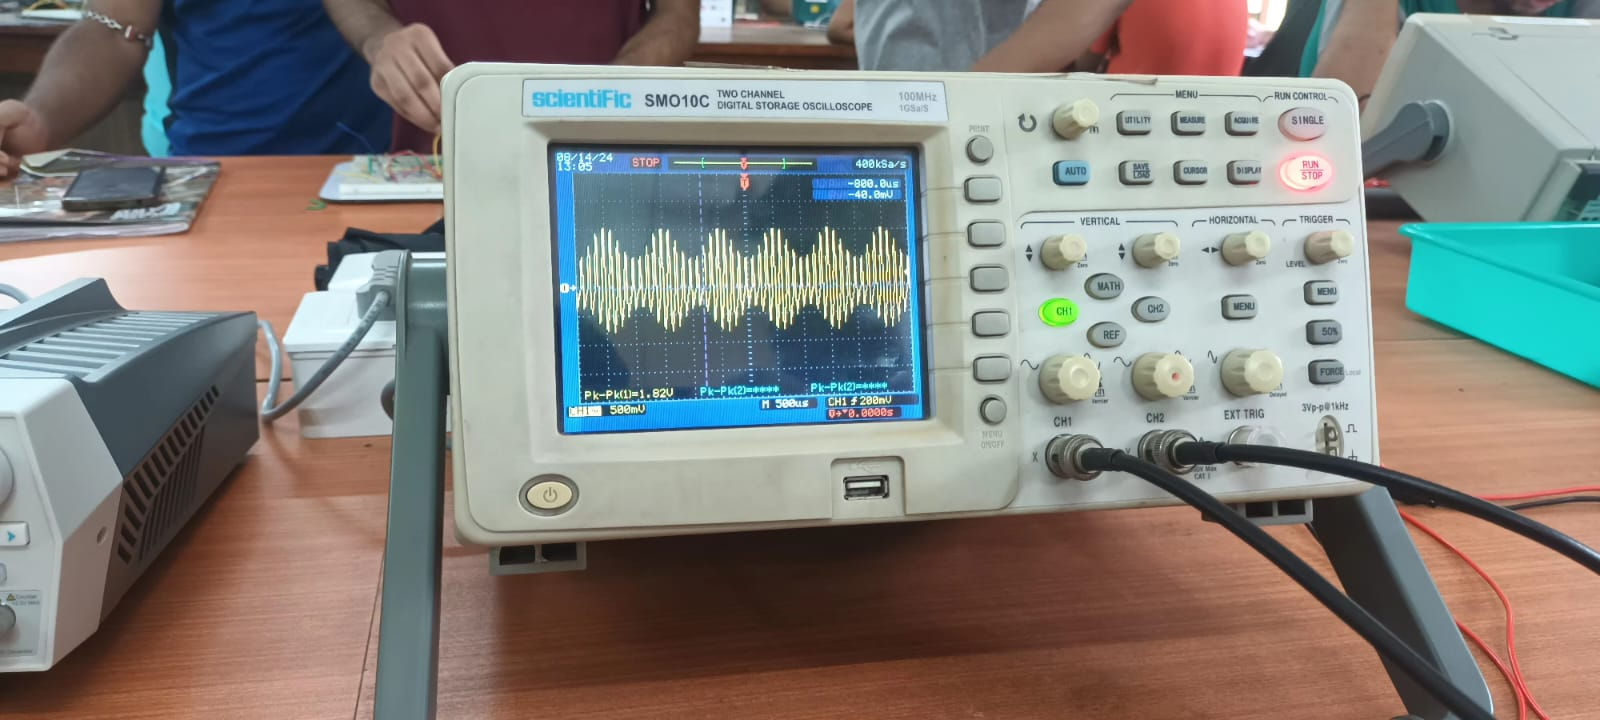
\includegraphics[width=\textwidth]{Modulated_signal.jpg}
\end{figure}
\newpage
\subsection{Task 2}
\begin{figure}[!ht]
  \caption{Demodulated signal in comparison with the original result}
  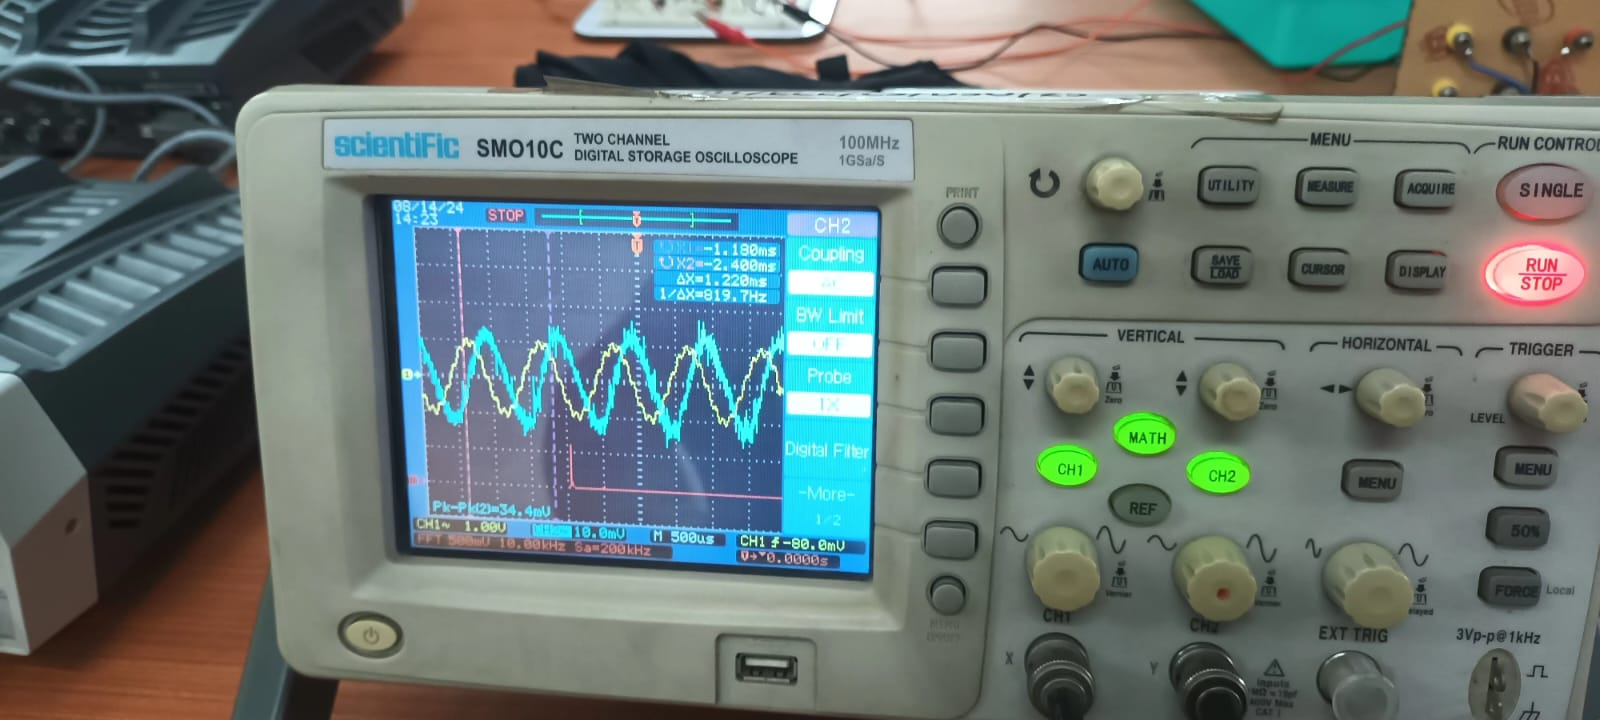
\includegraphics[width=\textwidth]{Demodulation_result.jpg}
\end{figure}


\section{Discussion}
\subsection{Samyak Sheersh, 22EC30045}
\begin{enumerate}
  \item When we didn't calibrate the demodulator circuit, we were able to see that the capacitor was charging and discharging noticeably slowly and thus the effects were visible on the envelope detected
  \item The final output is phase delayed, attenuated and still a bit noisy because at such small output voltages(~50mV), the background noise effects can be comparable. And since we made it pass through capacitive elements, there was a phase delay. We also didn't amplify the signal anywhere so the final output is in the 10s of mVs
  \item The initial signal as can be seen in the second picture is distorted because the high impedance isolating the signal generator wasn't strong enough and thus the loading due to the rest of the circuit caused it to distort.
  \item We also replaced the high R before the band pass filter with an op-amp buffer since that gave us a cleaner result as it was causing better isolation.
  \item We also discovered that there were no boundaries on the discharging time for the capacitor in the demodulator circuit except when the resistance got way too large and that led to parasitic capacitances and inductances of the material causing distortion to the final signal.
  \item The FFT of the modulated signal showed a peak at the $f_c$ with smaller peaks around $f_c\pm f_m$ 
\end{enumerate}
\end{document}

